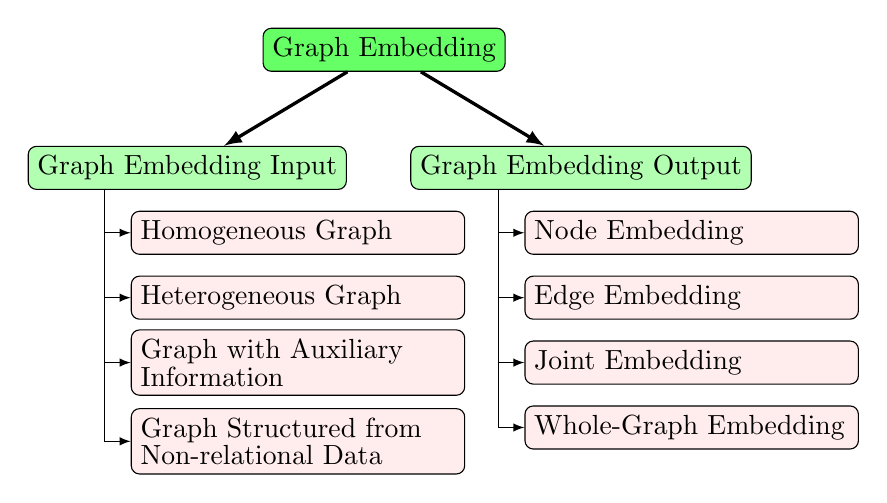
\begin{tikzpicture}[
	rec/.style  = {draw, rectangle, thin, execute at begin node=\setlength{\baselineskip}{1em}},
	root/.style = {rec, rounded corners=3pt,  fill=green!60},
	level 1/.style={sibling distance=50mm},
	level 2/.style={rec, rounded corners=3pt, fill=green!30},
	level 3/.style = {rec, rounded corners=3pt, align=left, fill=pink!30, text width=40mm, yshift=-10pt},
	edge from parent/.style={->,draw, very thick},
	>=latex]
	
	% root of the the initial tree, level 1
	\node[root] {Graph Embedding}
	child {node[level 2] (c1) {Graph Embedding Input}}
	child {node[level 2] (c2) {Graph Embedding Output}};
	
	% The second level, relatively positioned nodes
	\begin{scope}[every node/.style={level 3}]
		\node [below of = c1, xshift=40pt, yshift=15pt] (c11) {Homogeneous Graph};
		\node [below of = c11, yshift=15pt] (c12) {Heterogeneous Graph};
		\node [below of = c12, yshift=15pt] (c13) {Graph with Auxiliary Information};
		\node [below of = c13, yshift=10pt] (c14) {Graph Structured from Non-relational Data};
		
		\node [below of = c2, xshift=40pt, yshift=15pt] (c21) {Node Embedding};
		\node [below of = c21, yshift=15pt] (c22) {Edge Embedding};
		\node [below of = c22, yshift=15pt] (c23) {Joint Embedding};
		\node [below of = c23, yshift=15pt] (c24) {Whole-Graph Embedding};
	\end{scope}
	
	% lines from each level 1 node to every one of its "children"
	\foreach \value in {1,...,4}
	\draw[->] (c1.195) |- (c1\value.west);
	
	\foreach \value in {1,...,4}
	\draw[->] (c2.195) |- (c2\value.west);
\end{tikzpicture}